\chapter{Analiza FLUENT - rețele profile subțiri separate}\label{chapter:analiza}

Pentru a ne asigura că rezultatele obținute cu ajutorul calculelor proprii și cu ajutorul codului dezvoltat "in-house" de catedra de Mașini Hidraulice din Timișoara, dorim sa verificam rezultatele într-un software profesional dezvoltat pentru acest fel de aplicații, Gambit pentru discretizare și FLUENT pentru simularea numerica.

Analizăm așadar rezultatele obținute prin optimizare numerică și prin analiza în FLUENT pentru coeficientul de presiune pe cele doua profile separate.

\section{Rețele profile separate}

\subsection{Stator}

Pregătirea modelelor începe în Gambit unde aducem geometria profilului și construim banda de periodicitate. Pentru condițiile pe frontiera pregătim fetele geometriei 2D conform figurii 4.1.

\begin{figure}[h]
	\centering
	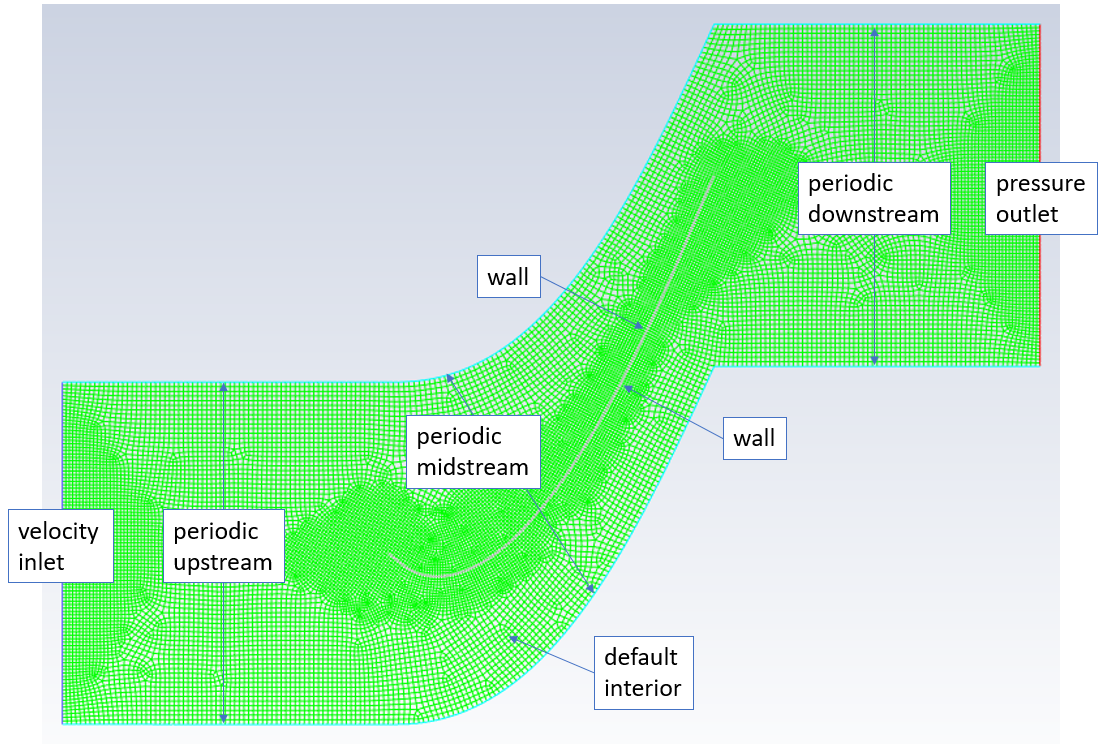
\includegraphics[scale=0.5]{figures/mesh-stator-boundary.PNG}
	\caption{Discretizare și condiții pe frontieră pentru stator în Gambit}
	\label{Discretizare și condiții pe frontieră pentru stator în Gambit}
\end{figure}

Coeficientul de presiune se calculează conform unui parametru "User-defined" introdus manual în ANSYS cu următoarea formula:

\begin{equation}
c_p = \frac{p-p_3}{\rho V_a^2 / 2}
\end{equation}

Valoarea absoluta pentru curgerea prin stator fiind:

\begin{equation}
= 1 + 2 \frac{V_{u2}}{V_a} \frac{U}{V_a} - {\frac{V}{V_a}}^2
\end{equation}

În figura 4.2. se poate vedea comparația intre rezultatele obținute numeric și rezultatele din Fluent pentru stator.

\begin{figure}[h]
	\centering
	\includegraphics[scale=0.4]{figures/cp-stator-ezdraw.eps}
	\caption{Coeficient de presiune stator - optimizare numerică / analiză FLUENT}
	\label{Coeficient de presiune stator - optimizare numerică / analiză FLUENT}
\end{figure}

\clearpage

\subsection{Rotor}

Analog simulării numerice pentru stator se procedează și pentru rotor. În Gambit sunt pregătite condițiile pe frontiera conform figurii 4.3. și se face discretizarea care urmează sa fie folosita apoi în Fluent.

\begin{figure}[h]
	\centering
	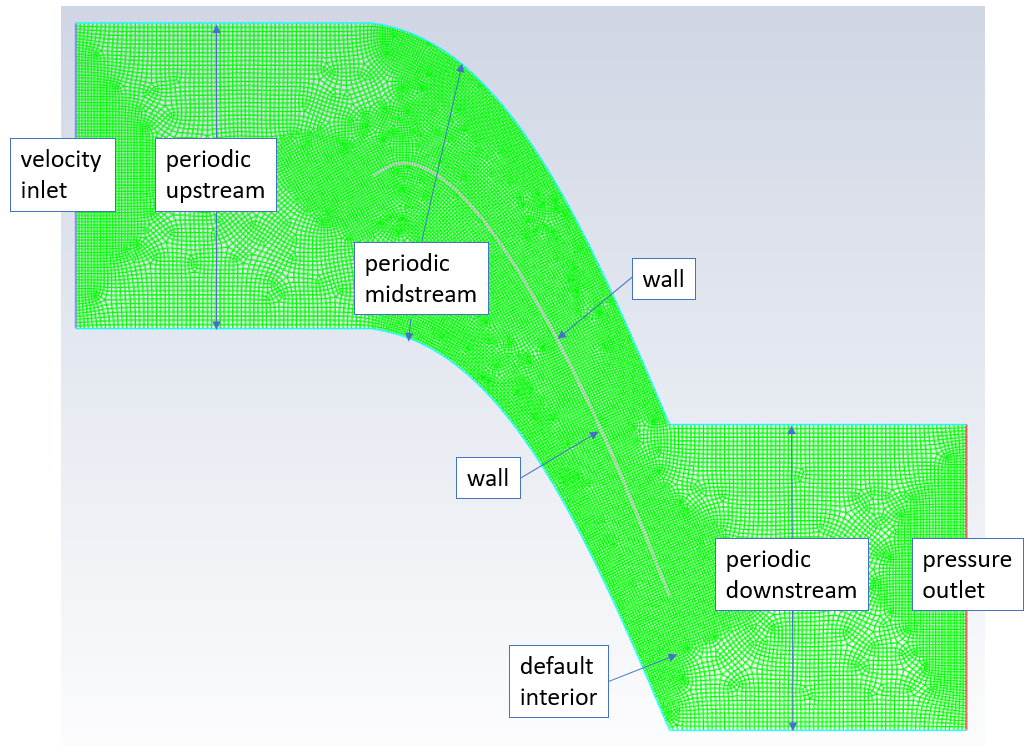
\includegraphics[scale=0.5]{figures/mesh-rotor-boundary.PNG}
	\caption{Discretizare și condiții pe frontieră pentru rotor în Gambit}
	\label{Discretizare și condiții pe frontieră pentru rotor în Gambit}
\end{figure}

Se poate observa în figura 4.4 că valorile obținute prin cele două metode, coeficient de presiune cu codul "in-house" precum și cu software-ul profesional ANSYS Fluent, sunt extrem de apropiate, lucru care ne validează rezultatele cu un anumit grad de siguranță, fără sa avem la îndemâna o validare experimentala.

Analog zonei statorului coeficientul de presiune se calculează conform unui parametru "User-defined" introdus manual în ANSYS cu următoarea formula pentru valoarea absoluta in rotor:

\begin{equation}
c_p = \frac{p-p_3}{\rho V_a^2 / 2} = 1 + 2 \frac{V_{u2}}{V_a} \frac{U}{V_a} - {\frac{V}{V_a}}^2
\end{equation}


\begin{figure}[t!]
	\centering
	\includegraphics[scale=0.4]{figures/cp-rotor-ezdraw.eps}
	\caption{Coeficient de presiune rotor - optimizare numerică / analiză FLUENT}
	\label{Coeficient de presiune rotor - optimizare numerică / analiză FLUENT}
\end{figure}

\clearpage

\section{Reprezentare analiză în tandem din FLUENT}

\begin{figure}[h]
	\centering
	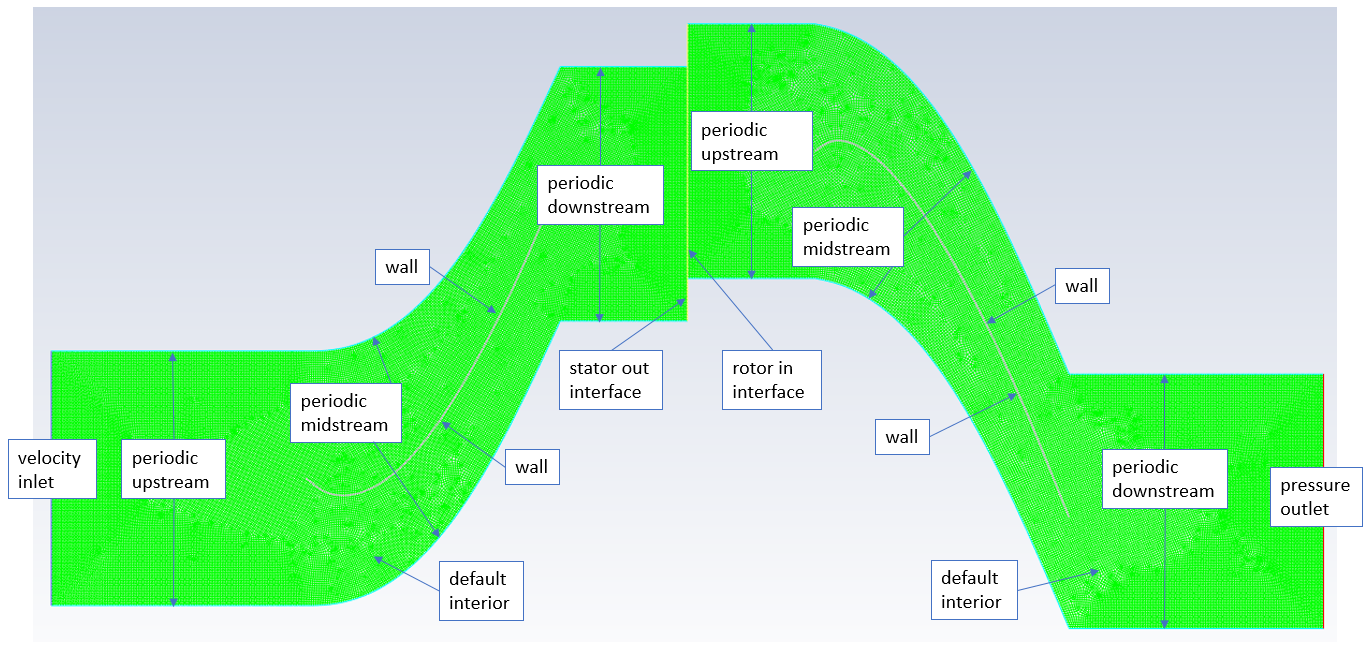
\includegraphics[scale=0.45]{figures/mesh-tandem-boundary.PNG}
	\caption{Discretizare și condiții pe frontieră pentru tandemul stator-rotor în Gambit}
	\label{Discretizare și condiții pe frontieră pentru tandemul stator-rotor în Gambit}
\end{figure}

\begin{figure}[!h]
	\centering
	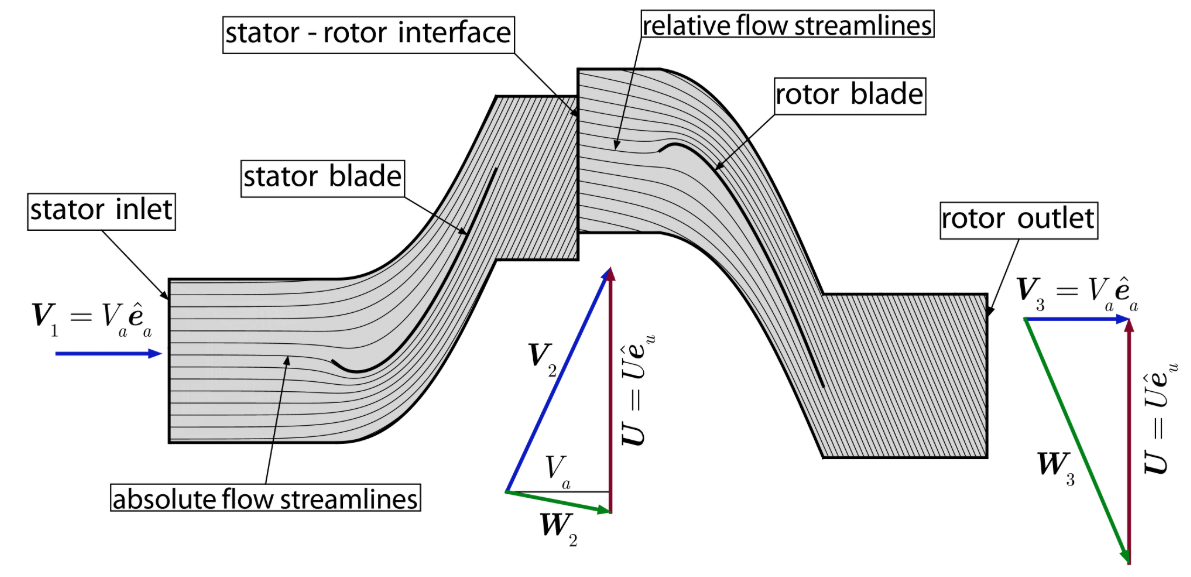
\includegraphics[scale=0.5]{figures/AXENT-tandem-streamlines.PNG}
	\caption{Reprezentare linii de curent în tandemul stator-rotor pentru turbina AXENT / analiză FLUENT}
	\label{Reprezentare linii de curent în tandemul stator-rotor pentru turbina AXENT / analiză FLUENT}
\end{figure}


În pregătirea simulării numerice pentru cele doua rețele de profile în tandem este nevoie de folosirea unei zone de interfață intre fata "stator out" și "rotor in" conform după cum se poate observa în figura 4.5. Restul condițiilor pe frontiera sunt asemănătoare pregătirii rețelelor de profile singulare în secțiunile precedente.

Cu ajutorul FLUENT în figura 4.6 se pot observa liniile de curent peste cele două profile precum și triunghiurile de viteze calculate inițial.

\clearpage